\def\duedate{09/30/22}
\def\HWnum{2}
% Document setup
\documentclass[12pt]{article}
\usepackage[margin=1in]{geometry}
\usepackage{fancyhdr}
\usepackage{lastpage}

\pagestyle{fancy}
\lhead{Richard Whitehill}
\chead{PHYS 675 -- HW \HWnum}
\rhead{\duedate}
\cfoot{\thepage \hspace{1pt} of \pageref{LastPage}}

% Encoding
\usepackage[utf8]{inputenc}
\usepackage[T1]{fontenc}

% Math/Physics Packages
\usepackage{amsmath}
\usepackage{mathtools}
\usepackage[arrowdel]{physics}
\usepackage{siunitx}

\AtBeginDocument{\RenewCommandCopy\qty\SI}

% Reference Style
\usepackage{hyperref}
\hypersetup{
    colorlinks=true,
    linkcolor=blue,
    filecolor=magenta,
    urlcolor=cyan,
    citecolor=green
}

\newcommand{\eref}[1]{Eq.~(\ref{eq:#1})}
\newcommand{\erefs}[2]{Eqs.~(\ref{eq:#1})--(\ref{eq:#2})}

\newcommand{\fref}[1]{Fig.~\ref{fig:#1}}
\newcommand{\frefs}[2]{Figs.~\ref{fig:#1}--\ref{fig:#2}}

\newcommand{\tref}[1]{Table~\ref{tab:#1}}
\newcommand{\trefs}[2]{Tables~\ref{tab:#1}-\ref{tab:#2}}

% Figures and Tables 
\usepackage{graphicx}
\usepackage{float}
\usepackage{booktabs}

\newcommand{\bef}{\begin{figure}[h!]\begin{center}}
\newcommand{\eef}{\end{center}\end{figure}}

\newcommand{\bet}{\begin{table}[h!]\begin{center}}
\newcommand{\eet}{\end{center}\end{table}}

% tikz
\usepackage{tikz}
\usetikzlibrary{calc}
\usetikzlibrary{decorations.pathmorphing}
\usetikzlibrary{decorations.markings}
\usetikzlibrary{arrows.meta}
\usetikzlibrary{positioning}

% tcolorbox
\usepackage[most]{tcolorbox}
\usepackage{xcolor}
\usepackage{xifthen}
\usepackage{parskip}

\newcommand*{\eqbox}{\tcboxmath[
    enhanced,
    colback=black!10!white,
    colframe=black,
    sharp corners,
    size=fbox,
    boxsep=8pt,
    boxrule=1pt
]}

% Miscellaneous Definitions/Settings
\newcommand{\prob}[2]{\textbf{#1)} #2}

\setlength{\parskip}{\baselineskip}
\setlength{\parindent}{0pt}
\setlength{\headheight}{14.49998pt}
\addtolength{\topmargin}{-2.49998pt}

\usepackage[compat=1.1.0]{tikz-feynman}

\begin{document}
    
\prob{1}{
The strong interactions are blind to flavor.
All quarks carry the same color charge.
Thus, the $\Sigma$ triplet of baryons, which all have identical wave functions, except for different numbers of $u$ and $d$ quarks, should have the same mass up to two effects: the electromagnetic energy, and the difference in mass between the $u$ and $d$ quark.
}

a) First, calculate the electromagnetic binding (or anti-binding) energy for each of these baryons, using the following simple model: Assume that the three quarks are, on average, each $\SI{1}{\femto\m}$ from each other in the $\Sigma$.
Express your answer in $\SI{}{\MeV}$.

The quark content of the $\Sigma$ baryons is listed below in \tref{sig-quarks}

\begin{table}[h!]
\begin{center}
\begin{tabular}{c|c}
    $Q$ & $qqq$ \\
    \hline
    $0$ & $uds$ \\
    $+$ & $uus$ \\
    $-$ & $dds$
\end{tabular}
\end{center}
\caption{Quark content of $\Sigma$ baryons by charge.}
\label{tab:sig-quarks}
\end{table}

The electric potential energy between charges $q_1$ and $q_2$ is given as $U(r) = q_1 q_2 / (4\pi\epsilon_0\langle r \rangle)$, so for an average separation distance of $\langle r \rangle = \SI{1}{\femto\m}$ we have
\begin{eqnarray}
    \label{eq:potential-energies}
    \eqbox{
    \begin{aligned}
    V_{\Sigma^{0}} &= \frac{q_{d} q_{s} + q_{d} q_{u} + q_{s} q_{u}}{4 \pi \epsilon_{0} \langle r \rangle} = \SI{-0.48}{\MeV} \\
    V_{\Sigma^{+}} &= \frac{q_{u} \left(2 q_{s} + q_{u}\right)}{4 \pi \epsilon_{0} \langle r \rangle} = \SI{0}{\MeV} \\
    V_{\Sigma^{-}} &= \frac{q_{d} \left(2 q_{s} + q_{d}\right)}{4 \pi \epsilon_{0} \langle r \rangle} = \SI{0.48}{\MeV} 
\end{aligned}
}
,\end{eqnarray}
Note that this is a classical analysis, defining the binding energy to be just the negative of the work done to assemble the charge distribution.


b) Just to get rid of gravity once and for all, calculate the gravitational binding energy for the three quarks in this model.
For simplicity, assume that each quark has about $1/3$ the mass of the $\Sigma$. \SI{}{\MeV} again.

The expressions above may be translated into a gravitational potential energy by taking $q \rightarrow m$ and $(4\pi\epsilon_0)^{-1} \rightarrow G$. 
Hence, we have (for $\langle r \rangle = \SI{1}{\femto\m}$ and $m_{u} = m_{d} = m_{s} = m_{\Sigma}/3$, where $m_{\Sigma}$ is the average mass of the $\Sigma$ baryons)
\begin{eqnarray}
    \label{eq:potential-energies-gravity}
    \eqbox{
        V = -\frac{G m_{\Sigma}^{2}}{3 \langle r \rangle} = \SI{-6.28e-37}{\MeV}
}
,\end{eqnarray}
which applies to all the $\Sigma$ baryons since we assume each quark flavor has the same mass as the others.
As is clearly seen here, this is a tiny binding energy.
Additionally, since mass differences come from different binding energies, the gravitational binding energy cannot produce any effect in the approximation we made above.
Even if we were more careful about using exact masses, however, the gravitational binding energy differences would still be orders of magnitude smaller than the $\SI{}{\MeV}$ scale that we care about.


c) Your answer to (a) may not be accurate, since we really do not know if \SI{1}{\femto\m} is the right distance.
However, the relative binding energies may be more reliable.
Use them and the three $\Sigma$ masses to solve for both the electromagnetic binding and the $d-u$ mass difference.

The masses of the $\Sigma$ baryons are given as follows:
\begin{align}
    \label{eq:masses_sigma}
    m_{\Sigma^{0}} &= m_{u} + m_{d} + m_{s} - V \\ 
    m_{\Sigma^{+}} &= 2m_{u} + m_{s} \\
    m_{\Sigma^{-}} &= 2m_{d} + m_{s} + V
,\end{align}
where $V = e^2/12\pi\epsilon_0\langle r \rangle$.
Since we have 3 equations, we can solve for $m_{u}$, $m_{d}$, and $V$ in terms of the $\Sigma$ baryon masses and $m_{s}$:
\begin{align}
    \label{eq:solve_system_sigma}
    m_{u} &= -\frac{m_{s} - m_{\Sigma^{+}}}{2}\\
    m_{d} &= -\frac{m_{s}}{2} - \frac{m_{\Sigma^{+}}}{6} + \frac{m_{\Sigma^{-}}}{3} + \frac{m_{\sigma^{0}}}{3} \\
    V &= \frac{m_{\Sigma^{+}} + m_{\Sigma^{-}} - 2m_{\Sigma^{0}}}{3}
.\end{align}

If we subtract the expression for the mass of the $d$ quark from that for the $u$ quark and plug in the masses of the $\Sigma$ baryons, we find
\begin{eqnarray}
    \label{eq:mass-diff_binding}
    \eqbox{
        \begin{aligned}
            m_{d} - m_{s} = -\frac{2m_{\Sigma^{+}} - m_{\Sigma^{-}} - m_{\Sigma^{0}}}{3} &= \SI{3.78}{\MeV} \\
            V &= \SI{0.51}{\MeV}
        \end{aligned}
}
.\end{eqnarray}
Note that this implies an average separation between the quarks of $\langle r \rangle = \SI{0.94}{\femto\m}$, which is not too far off of the \SI{1}{\femto\m} scale we assumed in part (a).


d) The $K^{0} - K^{\pm}$ mass difference is \SI{4.0}{\MeV / c^2} and the $B^{0} - B^{\pm}$ mass difference is \SI{0.33}{\MeV / c^2}.
Does this suggest to you that the $K$ mesons are larger or smaller in size than the $B$ mesons?

For the $K$ mesons we have
\begin{align}
    \label{eq:K-mass}
    m_{K^{0}} &= m_{d} + m_{s} - V_{K} \\
    m_{K^{\pm}} &= m_{u} + m_{s} + 2V_{K}
,\end{align}
where $V=e^2/36\pi\epsilon_0\langle r \rangle_{K}$, so the Kaon mass difference is given as
\begin{eqnarray}
    \label{eq:K-mass-diff}
    m_{K^{0}} - m_{K^{\pm}} = (m_{d} - m_{u}) + 3V_{K}
.\end{eqnarray}

For the $B$ mesons we have
\begin{align}
    \label{eq:B-mass} 
    m_{B^{0}} &= m_{d} + m_{b} - V_{B} \\
    m_{B^{\pm}} &= m_{u} + m_{b} + 2V_{B}
,\end{align}
and as in the case with kaons
\begin{eqnarray}
    \label{eq:B-mass-diff}
    m_{B^{0}} - m_{B^{\pm}} = (m_{d} - m_{u}) - 3V_{B}
.\end{eqnarray}


\prob{2}{
Classically, light cannot scatter from light, but it is allowed by relativistic quantum mechanics.
Called Delbr\"{u}ck scattering, after the physicist who predicted it in 1933, it was first observed in 1953 by R.R. Wilson.
Draw the lowest-order Feynman diagram for Delbr\"{u}ck scattering.
}

We know that photons, which are chargeless, cannot interact directly via the electromagnetic interaction.
However, they may produce virtual charged fermion-antifermion pairs (e.g. $e^{+}e^{-}$) that interact with each other, allowing the photons to indirectly interact with each other via the electromagnetic force.
The lowest order diagram is shown below.

\begin{figure}[H]
\begin{center}
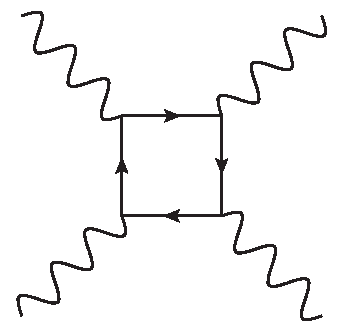
\includegraphics[width=0.3\textwidth]{prob2/prob2.pdf}
\end{center}
\caption{Lowest order feynman diagram for $\gamma\gamma$ interactions. Note that we could draw similar diagrams by interchanging adjacent photon vertices.}
\label{fig:delbruck-diagram}
\end{figure}


\prob{3}{
In $e^{+}e^{-}$ annihilation experiments, a second process occurs in which the electron and positron do not annihilate, but produce a fermion-antifermion pair by the exchange of two photons, as shown to the right.
}

\begin{figure}[H]
\begin{center}
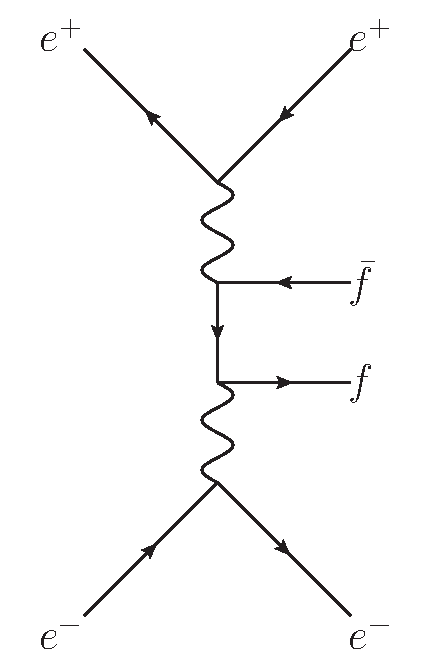
\includegraphics[width=0.3\textwidth]{prob3/prob3_graph.pdf}
\end{center} 
\caption{Feynman diagram for $e^{+}e^{-} \rightarrow e^{+}e^{-}\bar{f}f$ without annihilation of the initial state $e^{+}e^{-}$ particles.}
\label{fig:prob3-fig}
\end{figure}

(a) For very high energy, and for a very high mass fermion-antifermion pair (these conditions allow you to ignore the mass of the fermions in your calculation), what do you expect for the ratio
\begin{eqnarray}
    \label{eq:ratio}
    R = \frac{\sigma(e^{+}e^{-} \rightarrow e^{+}e^{-}{\rm hadrons})}{\sigma(e^{+}e^{-} \rightarrow e^{+}e^{-}\mu^{+}\mu^{-})}
.\end{eqnarray}
Use $u$, $d$, $s$, $c$, and $b$ quarks in your calculation (The world does not have an $e^{+}e^{-}$ colliding beam facility that works at high enough energy to include $t$ quarks).

For the reaction $e^{+}e^{-} \rightarrow e^{+}e^{-}f\overline{f}$, the difference in the squared amplitudes for different fermions $f$ only arises from differences in the vertex factors where $f$ and $\overline{f}$ are produced, which is where the charge of the fermion, $e_{f}$, appears.
For quarks, we have 
\begin{eqnarray}
    \label{eq:sigma-quarks}
    \sigma(e^{+}e^{-} \rightarrow e^{+}e^{-}q\overline{q}) \propto 3\sum_{q} e_{q}^4
,\end{eqnarray}
while for $\mu^{+}\mu^{-}$ production
\begin{eqnarray}
    \label{eq:sigma-mu}
    \sigma(e^{+}e^{-} \rightarrow e^{+}e^{-}\mu^{+}\mu^{-}) \propto e^4
.\end{eqnarray}
Hence,
\begin{eqnarray}
    \label{eq:ratio-calculation}
    \eqbox{
    R = 3 \sum_{q} \Big( \frac{e_{q}}{e} \Big)^2 = 3\Big[3\Big(-\frac{1}{3}\Big)^4 + 2\Big(\frac{2}{3}\Big)^4\Big] = \frac{1}{27}(3 + 32) = \frac{35}{27}
}
.\end{eqnarray}



(b) There are several other electromagnetic diagrams of the same order that lead to the identical final state, but would give a different answer than you have just calculated.
Draw one of them. (Hint: let the $e^{+}e^{-}$ annihilate.)
(Note that since these are indistinguishable processes, the amplitudes have to be added before squaring.
In most cases, the diagram for part (a) dominates, so your answer in part (a) is close to correct for the stated conditions.)

If we have the electron and positron annihilate then we may have a diagram of the same order as \fref{prob3-fig} like the one shown in \fref{prob3-same-order}.

\begin{figure}[H]
\begin{center}
    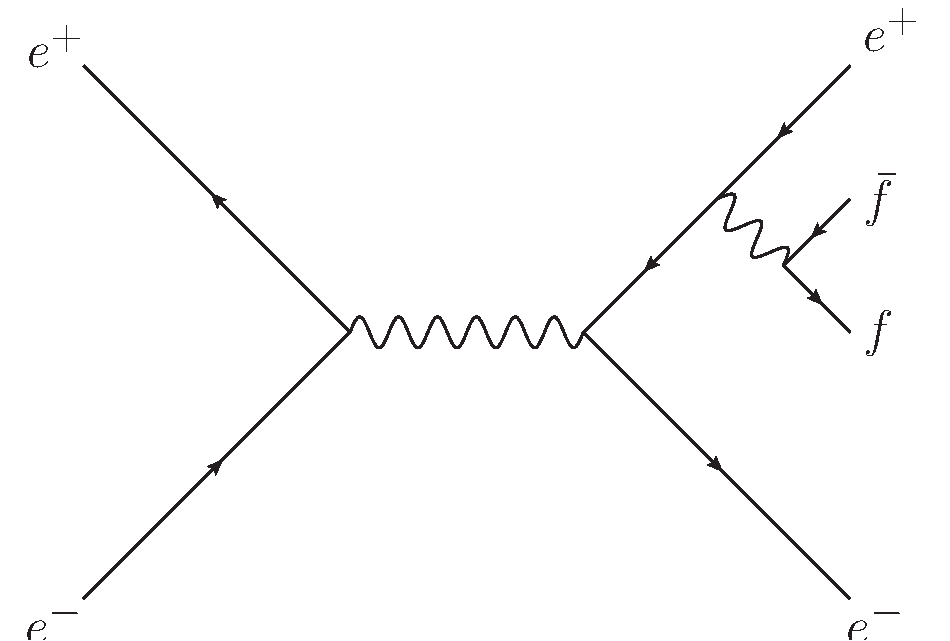
\includegraphics[width=0.6\textwidth]{prob3/prob3.pdf}    
\end{center}
\caption{Diagram for $e^{+}e^{-} \rightarrow e^{+}e^{-}f\overline{f}$ process of the same order as \fref{prob3-fig}. Note that the labels of $f$ and $e$ may be interchanged in the final state and the virtual photon line could have been drawn coming off of the lower leg of the final state fermion as well.}
\label{fig:prob3-same-order}
\end{figure}


\prob{4}{
Consider the following possible decays and reactions.
If the reaction is forbidden, state what conservation law is violated. 
(Don't forget to check energy conservation for the decays.
For the reactions, you can assume that there is enough energy in the initial state to make the reaction go.)
If the reaction or decay is allowed, draw a diagram showing the leading mechanism, (i.e. strong, if possible, otherwise electromagnetic, if possible, otherwise weak).
}

(a) $e^{+}e^{-} \rightarrow \tau^{+}\tau^{-}$

This is an allowed electromagnetic process.

\begin{center}    
\begin{tikzpicture}
\begin{feynman}
   \vertex (O) at (0,0);
   \vertex[right=of O] (pr);
   \vertex[left=of O] (pl);
   \vertex[above left=of pl] (ep) {$e^{+}$};
   \vertex[below left=of pl] (en) {$e^{-}$};
   \vertex[above right=of pr] (tp) {$\tau^{+}$};
   \vertex[below right=of pr] (tn) {$\tau^{-}$};

   \diagram* {
    (pl) -- [photon] (pr),
    (ep) -- [anti fermion] (pl),
    (en) -- [fermion] (pl),
    (pr) -- [anti fermion] (tp),
    (pr) -- [fermion] (tn),
   };

\end{feynman}
\end{tikzpicture}
\end{center}

\begin{figure}[H]
\begin{center}
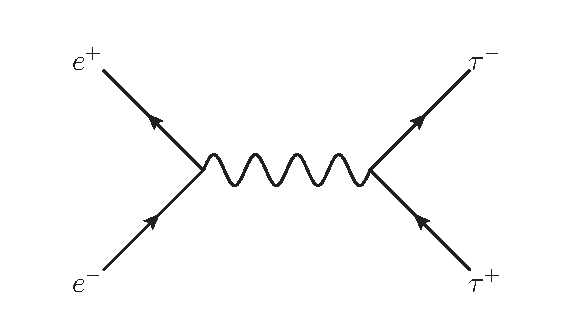
\includegraphics[width=0.5\textwidth]{prob4/a.eps} 
\end{center} 
\end{figure}

(b) $e^{+}e^{-} \rightarrow \pi^{+}\pi^{-}$

This is an allowed process.
The photon coming off the $u$ quark could also be a gluon line.

\begin{figure}[H]
\begin{center}
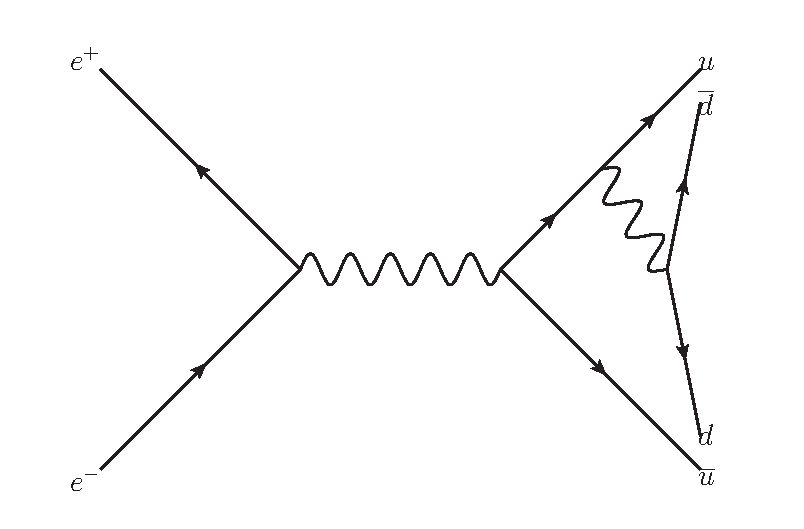
\includegraphics[width=0.5\textwidth]{prob4/b.eps} 
\end{center} 
\end{figure}

(c) $e^{-}p \rightarrow e^{-}n\pi^{+}$ 

This is an allowed strong process.

(d) $e^{-}p \rightarrow \nu_{e}n\pi^{0}$

(e) $\nu_{\mu}e^{-} \rightarrow \nu_{e}\mu^{-}$

(f) $\overline{\nu}_{\mu}e^{-} \rightarrow \overline{\nu}_{e}\mu^{-}$

(g) $\overline{\nu}_{e}e^{-} \rightarrow \pi^{-}\pi^{0}$

(h) $\overline{\nu}_{e}e^{-} \rightarrow \nu_{e}e^{+}$ 

(i) $\pi^{+}n \rightarrow p\gamma$

(j) $e^{+}e^{-} \rightarrow \nu_{\mu}\overline{\nu}_{\mu}$

(k) $p\overline{p} \rightarrow \Sigma^{+}\Sigma^{-}$

(l) $\pi^{+}n \rightarrow \Lambda K^{+}$

(m) $\tau^{-} \rightarrow K^{-}\nu_{\tau}$

(n) $\Sigma^{0} \rightarrow \Lambda \pi^{0}$

(o) $\psi \rightarrow \rho^{+}\pi^{-}$

(p) $\pi^{+} \rightarrow e^{+}\nu_{e}$

(q) $\Omega^{-} \rightarrow \Xi^{0}K^{-}$

(r) $\Omega^{-} \rightarrow \Lambda K^{-}$

(s) $n \rightarrow e^{-}\overline{\nu}_{e}\pi^{+}$

(t) $B^{-} \rightarrow \psi K^{-}$


\prob{5}{
The second charmed particle to be discovered, the $D^{+}$, was found first in the decay mode $D^{+} \rightarrow K^{-}\pi^{+}\pi^{+}$.
}

(a) Draw a diagram for this decay.

%\begin{figure}
%\begin{center}
%\begin{tikzpicture}
%\begin{feynman}
%    
%\end{feynman}    
%\end{tikzpicture}    
%\end{center} 
%\end{figure}

(b) Ignoring its narrow width, the experimenters who discovered this mode knew immediately that it could not come from the strong decay of a meson.
Why?

Writing the decay in terms of quark content we have
\begin{eqnarray}
    \label{eq:decay-quark}
    c \overline{d} \rightarrow s \overline{u} + u \overline{d} + u \overline{d}
.\end{eqnarray}
Obviously, flavor is not conserved in this decay, but the strong force conserves quark flavor in any process.
So this decay cannot proceed strongly.

\prob{6}{
The decays $D^{0} \rightarrow K^{-}\pi^{+}$ and $D^{0} \rightarrow K^{+}\pi^{-}$ are both allowed.
However, the former has a much higher branching ratio than the latter.
Draw the diagrams for these two decays and estimate the ratio of branching fractions due to the Cabibo mixing angle factors.
Compare your answer to the data summary in the PDG tables.
}



\end{document}
